\chapter{The electric potential}

\section{Line integral of the electric field}\index{electric field!line integral of}
Suppose that $\vc{E}$ is the field of some stationary distribution of electric
charges. Let $P_1$ and $P_2$ denote two positions anywhere in the
field. The line integral of $\vc{E}$ between the two given points is 
$\int_{P_1}^{P_2}\vc{E}\cdot\der\vc{s}$,
taken along some path that runs from $P_1$ to $P_2$, as in Fig. 2.1. This
means: Divide the path into short segments, each segment being
represented by a vector connecting its ends; take the scalar product
of the path-segment vector with the field $\vc{E}$ at that place; add these
products up for the whole path. The integral as usual is to be 
regarded as the limit of this sum as the segments are made shorter and
more numerous without limit.

Let's work out a concrete example. Suppose we have an electric
field $\vc{E}$ such that $E_x = Ky$ and $E_y = Kx$, where K is a constant. This
happens to be a possible form for an electrostatic field. (We shall
learn presently how that can be quickly recognized.) Figure 2.2a
shows some field lines. What is the value of the line integral of $\vc{E}$,
between point $A$ and point $C$, over the particular path $ABC$ in the
diagram? The vector which represents a path element is
\begin{equation}
  \der \vc{s} = \hat{\vc{x}} \der x + \hat{\vc{y}} \der y
\end{equation}
and since the vector $\vc{E}$ is here
\begin{equation}
  \vc{E} = K(\hat{\vc{x}} y + \hat{\vc{y}} x)
\end{equation}
the scalar product $\vc{E}\cdot\der\vc{s}$ for any element of the path is
\begin{equation}
  \vc{E}\cdot\der\vc{s} = K(y\der x + x\der y)
\end{equation}
Along the portion of the path from $A$ to $B$, $y = 2x$ and $\der y = 2 dx$.
Therefore:
\begin{equation}
  \int_A^B \vc{E}\cdot\der\vc{s} = K\int_A^B  (y\der x+x\der y)
         = K\int_0^1(2x\der x+2x\der x)
         = 4K\int_0^1 x \der x = 2K
\end{equation}
Along the path from $B$ to $C$, $y = 2$ and $\der y = 0$.
\begin{equation}
  \int_B^C \vc{E}\cdot\der\vc{s} = K \int_B^C(y\der x+x\der y) = K\int_1^22\der x = 2K
\end{equation}
The line integral over the path $ABC$ is, therefore, $2K + 2K$, or $4K$.
% p. 37
The electric field of a point charge is directed radially and its magnitude
depends only on the radius $r$. If $P_1$ and $P_2$ are any two points
in the field of a point charge, it is pretty obvious that the line integral
of $\vc{E}$ is the same for all paths connecting these points. That follows
directly from the argument we used in Sec. 1.5, illustrated by Fig. 1.5,
for the work done when a charge is moved in a central field of force.
In fact, the only difference between the line integral of the force $\vc{F}$ on
a test charge q and the line integral of $\vc{E}$, the field through which the
test charge is moved, is the factor $q$. Now any electrostatic field is
simply the superposition of the fields of certain charges, as expressed
in Eqs. 1.14 and 1.15. In any such field, therefore, the line integral
of $\vc{E}$, the total $\vc{E}$ due to all the sources, must be path-independent:
\begin{equation}
\boxed{
  \int_{P_1}^{P_2} \vc{E}\cdot\der\vc{s} \text{has the same value for all paths connecting
       $P_1$ and $P_2$, in an electrostatic field}
}
\end{equation}

As an illustration, consider the line integral from $A$ to $C$ in Fig. 2.2c,
over the path via the point $(2,0)$, the field $\vc{E}$ being the same as before.
Along the first portion, the $x$ axis between the origin and $x = 2$, the
field is perpendicular to the path, so $\vc{E}\cdot\der\vc{s}$ is zero. On the second leg,
$E_y = Kx = 2K$, and the length of that path is 2 units. We get for the
line integral, then, $4K$; the same as before. In fact, once we recognize
that the line integral must be path-independent, it seems foolish to
evaluate it for a path like $ABC$. Actually, we shall not often need to
compute the value of a line integral. The main purpose of the example
is to make sure you understand what the line integral means.

\section{Potential difference and the potential function}
Because the line integral in the electrostatic field is path-
independent, we can use it to define a scalar quantity $\pot_{21}$, as follows:
\begin{equation}
\boxed{
  \pot_{21} = -\int_{P_1}^{P_2} \vc{E}\cdot\der\vc{s}
}
\end{equation}
Then $\pot_{21}$ is the \emph{work per unit charge} done in moving a positive
charge from $P_1$ to $P_2$ in the field $\vc{E}$. Thus $\pot_{21}$ is a single-valued scalar
function of the two positions $P_1$ and $P_2$. We call it the electric
\emph{potential difference}\index{potential|see{electric potential}}\index{electric potential!difference}
between the two points.

In our CGS system of units, potential difference is measured in
ergs/esu. This unit has a name of its own, the \intro{statvolt} (the ``stat''
% p. 38
comes from ``electrostatic''). The volt is the unit of potential difference
in the MKS system.\footnote{Like the coulomb, ampere, and
ohm, the volt was in common use as a ``practical''
electrical unit long before the complete MKS system of electrical units was contrived.}
It is equivalent to 1/299.79, approximately
1/ 300, of a statvolt. One joule ($10^7$ ergs) of work is required
to move a charge of one coulomb through a potential difference of
one volt.

Suppose we hold $P_1$ fixed at some reference position. Then $\pot_{21}$
becomes a function of $P_2$ only, that is, a function of the spatial coordinates
$x$, $y$, $z$. We can write it simply $\pot(x,y,z)$, without the sub-
scripts, if we remember that its definition still involves agreement
on a reference point $P_1$. We say that $\pot$ is the potential associated with
the vector field $\vc{E}$. It is a scalar function of position, or a scalar field
(they mean the same thing). Its value at a point is simply a number
(in units of work per unit charge) and has no direction associated
with it. Once the vector field $\vc{E}$ is given, the potential function $\pot$
is determined, except for an arbitrary additive constant allowed by
the arbitrariness in our choice of $P_1$.

As an example, let us find the potential associated with the electric
field described in Fig. 2.2. It is convenient to locate $P_1$ at the origin,
the point labeled $A$ in Fig. 2.2. To evaluate
\begin{equation}
  \int\vc{E}\cdot\der\vc{s}
\end{equation}
from this reference point to a general point $(x,y)$ it is easiest to use
a path like the dotted path in Fig. 2.2c:
\begin{equation}
  \pot(x,y) = -\int_{(0,0)}^{(x,y)}\vc{E}\cdot\der\vc{s}
            = -\int_{(0,0)}^{(x,0)} E_x \der x - \int_{(x,0)}^{(x,y)} E_y \der y
\end{equation}
The first integral is zero, as we noted earlier, because in this field $E_x$
is zero along the $x$ axis. The second integration is carried out at constant
$x$, and since $E_y = Kx$, the integral becomes
\begin{equation}
  -Kx\int_0^y \der y
\end{equation}
which has the value $-Kxy$. For this field then, the potential is
\begin{equation}
  \pot = -Kxy
\end{equation}
Any constant could be added to this. That would only mean that the
reference point to which zero potential is assigned had been located
somewhere else.

% p. 39
We must be careful not to confuse the potential $\pot$ associated with
a given field $\vc{E}$ with the \emph{potential energy} of a system of charges. The
potential energy of a system of charges is the total work required to
assemble it. In Eq. 1.8, for example, we expressed $U$, the potential
energy of the charge system in Fig. 1.6. The electric \emph{potential}\index{electric potential!defined}
$\pot(x,y,z)$ associated with the field in Fig. 1.6 would be the work per
unit charge required to bring a unit positive test charge in from infinity
to the point $(x,y,z)$ in the field of that structure of eight charges.

\section{Gradient of a scalar function}

Given the electric field, we can find the electric potential function.
But we can also proceed in the other direction; from the potential we
can derive the field. It would appear from Eq. 7 that the field is in
some sense the \emph{derivative} of the potential function. To make this idea
precise we introduce the \intro{gradient} of a scalar function of position.
Let $f(x,y,z)$ be some continuous, differentiable function of the co-
ordinates. With its partial derivatives $\partial f/\partial x$, 
$\partial f/\partial y$, and $\partial f/\partial z$,  we
can construct at every point in space a vector, the vector whose $x$, $y$, $z$
components are equal to the respective partial derivatives.\footnote{We
remind the reader that a partial derivative with respect to $x$, of a function of
$x$, $y$, $z$:, written simply $\partial f/\partial x$,
means the rate of change of the function with respect to $x$
with the other variables $y$ and $z$ held constant. More precisely,
\begin{equation*}
  \frac{\partial f}{\partial x} = \lim_{\Delta x\rightarrow0} \frac{f(x+\Delta x,y,z)-f(x,y,z)}{\Delta x}
\end{equation*}
As an example, if $f = x^2yz^3$,
\begin{equation*}
  \partial f/\partial x=2xyz^3 \qquad \partial f/\partial y=x^2z^3 \qquad \partial f/\partial z = 3x^2yz^2
\end{equation*}
} This
vector we call the \emph{gradient} of $f$, written $\operatorname{grad} f$, or $\grad f$.
\begin{equation}
\boxed{
  \grad f = \xhat \frac{\partial f}{\partial x} + \yhat \frac{\partial f}{\partial y}
          + \zhat \frac{\partial f}{\partial z}
}
\end{equation}
\noindent $\grad f$ is a vector that tells how the function $f$ varies in the neighborhood
of a point. Its $x$ component is the partial derivative off with respect
to $x$, a measure of the rate of change of $f$ as we move in the $x$ direction.
The direction of the vector $\grad f$ at any point is the direction in which
one must move from that point to find the most rapid increase in the
function $f$. Suppose we were dealing with a function of two variables
only, $x$ and $y$, so that the function could be represented by a surface
in three dimensions. Standing on that surface at some point, we see
% p. 40
the surface rising in some direction, sloping downward in the opposite
direction. There is a direction in which a short step will take us
higher than a step of the same length in any other direction. The
gradient of the function is a vector in that direction of steepest ascent
and its magnitude is the slope, measured in that direction.

Figure 2.3 may help you to visualize this. Suppose some particular
function of two coordinates $x$ and $y$ is represented by the surface
$f(x,y)$ sketched in Fig. 2.3a. At the location $(x_1,y_1)$ the surface rises
most steeply in a direction that makes an angle of about $80\degunit$ with the
positive $x$ direction. The gradient of $f(x,y)$, $\grad f$, is a vector function
of $x$ and $y$. Its character is suggested in Fig. 2.3b by a number of
vectors at various points in the two-dimensional space, including the
point $(x_1,y_1)$. The vector function $\grad f$ defined in Eq. 12 is simply an
extension of this idea to three-dimensional space. [Be careful not to
confuse Fig. 2.3a with real three-dimensional $xyz$ space; the third
coordinate there is the value of the function $f(x,y)$.]

As one example of a function in three-dimensional space, suppose
$f$ is a function of $r$ only where $r$ is the distance from some fixed
point $O$. On a sphere of radius $r_0$ centered about $O$, $f = f(r_0)$ is
constant. On a slightly larger sphere of radius $r_0 + \der r$ it is also con-
stant, with the value $f = f(r_0 + \der r)$. If we want to make the change
from $f(r_0)$ to $f(r_0 + \der r)$, the shortest step we can make is to go
radially (as from $A$ to $B$) rather than from $A$ to $C$, in Fig. 2.4. The
``slope'' off is thus greatest in the radial direction, so $\grad f$ at any point
is a radially pointing vector. In fact $\grad f = \hat{\vc{r}} (\der f/\der r)$ in this case,
$\rhat$ denoting, for any point, a unit vector in the radial direction.

\section{Derivation of the field from the potential}\index{electric field!derived from potential}

It is now easy to see that the relation of the scalar function f to the
vector function $\grad f$ is the same, except for a minus sign, as the relation
of the potential $\pot$ to the field $\vc{E}$. Consider the value of $\pot$ at two nearby
points, $(x,y,z)$ and $(x + \der x, y + \der y, z + \der z)$. The change in $\pot$, going
from the first point to the second, is
\begin{equation}
  \der \pot = \frac{\partial\pot}{\partial x} \der x 
            + \frac{\partial\pot}{\partial y} \der y
            + \frac{\partial\pot}{\partial z} \der z + 
\end{equation}
On the other hand, from the definition of $\pot$, the change can also be
expressed as
\begin{equation}
  \der\pot = -\vc{E}\cdot\der\vc{s}
\end{equation}
% p. 41
The infinitesimal vector displacement $\der\vc{s}$ is just $\xhat\der x+\yhat\der y+\zhat\der z$.
Thus if we identify $\vc{E}$ with $-\grad\pot$, Eqs. 13 and 14 become identical. So
the electric field is the negative of the gradient of the potential:
\begin{equation}
\boxed{
  \vc{E}=-\grad\pot
}
\end{equation}
\noindent The minus sign came in because the electric field points from a region
of positive potential toward a region of negative potential, whereas
the vector $\grad\pot$ is defined so that it points in the direction of increasing
$\pot$.

To show how this works, we go back to the example of the field in
Fig. 2.2. From the potential given by Eq. 11, $\pot = -Kxy$, we can
recover the electric field we started with:
\begin{equation}
  \vc{E} = -\grad(-Kxy)
         =-\left(\xhat\frac{\partial}{\partial x}+\yhat\frac{\partial}{\partial y}+\right)(-Kxy)
         =K(\xhat y+\yhat x)
\end{equation}

\section{Potential of a charge distribution}\index{electric potential!of a continuous charge distribution}

We already know the potential that goes with a single point charge,
because we calculated the work required to bring one charge into the
neighborhood of another in Eq. 3. The potential at any point, in the
field of an isolated point charge $q$, is just $q/r$, where $r$ is the distance
from the point in question to the source $q$, and where we have
assigned zero potential to points infinitely far from the source.

Superposition must work for potentials as well as fields. If we
have several sources, the potential function is simply the sum of the
potential functions that we would have for each of the sources present
alone---\emph{providing} we make a consistent assignment of the zero of
potential in each case. If all the sources are contained in some finite
region, it is always possible, and usually the simplest choice, to put
zero potential at infinite distance. If we adopt this rule, the potential
of any charge distribution can be specified by the integral:
\begin{equation}
  \pot(x,y,z) = \int_{\text{All sources}} \frac{\rho(x',y',z')\der x'\der y'\der z'}{r}
\end{equation}
where $r$ is the distance from the volume element $\der x'\der y'\der z'$ to the
point $(x,y,z)$, at which the potential is being evaluated (Fig. 2.5).
That is, $r = [(x - x')^2 + (y - y')^2 + (z - z')^2]^{1/2}$. Notice the
difference between this and the integral giving the electric field of a
% p. 42
charge distribution, Eq. 1.15. Here we have $r$ in the denominator,
not $r^2$, and the integral is a scalar not a vector. From the scalar potential
function $\pot(x,y,z)$ we can always find the electric field by taking
the negative gradient of $\pot$, according to Eq. 15.

\subsection{Potential of two point charges}

 Consider a very simple example,
the potential of the two point charges shown in Fig. 2.6. A positive
charge of 12 esu is located 3 cm away from a negative charge, $- 6$ esu.
The potential at any point in space is the sum of the potentials due to
each charge alone. The potentials for some selected points in space
are given in the diagram. No vector addition is involved here, only
the algebraic addition of scalar quantities. For instance, at the point
on the far right which is 6 cm from the positive charge and 5 cm from
the negative charge, the potential has the value $\frac{+12}{6}+\frac{-6}{5}=+0.8$.
The unit here comes out esu/cm, which is the same as ergs/esu, or
\emph{statvolts}. The potential approaches zero at infinite distance. It
would take 0.8 erg of work to bring a unit positive charge in from
infinity to a point where $\pot = 0.8$ statvolt. Note two of the points
shown on the diagram have $\pot = O$. The net work done in bringing
in any charge to one of these points would be zero. You can see that
there must be an infinite number of such points, forming a surface in
space surrounding the negative charge. In fact the locus of points
with any particular value of $\pot$ is a surface, called an \intro{equipotential
surface}, which would show on our two-dimensional diagram as a
curve.

\subsection{Potential of a long charged wire}

There is one restriction on the
use of Eq. 17: It may not work unless all sources are confined to some
finite region of space. A simple example of the difficulty that arises
with charges distributed out to infinite distance is found in the long
charged wire whose field $\vc{E}$ we studied in Sec. 1.12. If we attempt to
assign zero potential to remote points in that system, and carry out
the integration over the charge distribution indicated in Eq. 15, we
find that the integral diverges---we get an infinite result. We might
have expected trouble, because in this case ``infinity,'' that is, all of
space very far from the region in which we wish to define a potential
function, contains not only points remote from the wire but most of
the wire itself! No such difficulty arose in finding the electric \emph{field} of
the infinitely long wire, because the contributions of elements of the
line charge to the field decrease so rapidly with distance. Evidently
we had better locate the zero of potential somewhere close to home,
% p. 43
in a system which has charges distributed out to infinity. Then it is
simply a matter of calculating the difference in potential $\pot_{21}$, between
the general point $(x,y,z)$ and the selected reference point, using the
fundamental relation, Eq. 7.

To see how this goes in the case of the infinitely long charged wire,
let us arbitrarily. locate the reference point $P_1$ at a distance $r_1$ from
the wire. Then to carry a charge from $P_1$ to any other point $P_2$ at
distance $r_2$ requires the work per unit charge
\begin{equation}
  \pot_{21} = -\int_{P_1}^{P_2} \vc{E}\cdot\der\vc{s}
            = -\int_{r_1}^{r_2} \left(\frac{2\lambda}{r}\right)
            = -2\lambda\ln r_2 + 2\lambda \ln r_1
\end{equation}
This shows that the electrical potential for the charged wire can be
taken as
\begin{equation}
  \pot = -2\lambda\ln r + \text{const}
\end{equation}
The constant, $2\lambda\ln r_1$ in this case, has no effect when we take $-\grad\pot$
to get back to the field $\vc{E}$. In this case,
\begin{equation}
  -\grad\pot = -\rhat\frac{\der\pot}{\der r} = \frac{2\lambda\rhat}{r}
\end{equation}


\section{Uniformly charged disk}

Let us study, as a concrete example, the electric potential and field
around a uniformly charged disk. This is a charge distribution like
that discussed in Sec. 1.10, except that it has a limited extent. The
flat disk of radius $a$ in Fig. 2.7 carries a positive charge spread over its
surface with the constant density $\sigma$, in $\esu/\cmunit^2$. (This is a single sheet
of charge of infinitesimal thickness, not two layers of charge, one on
each side. That is, the total charge in the system is $\pi a^2\sigma$.) We shall
often meet surface charge distributions in the future, especially on
metallic conductors. However the object just described is not a con-
ductor; if it were, as we shall soon see, the charge could not remain
uniformly distributed but would redistribute itself, crowding more
toward the rim of the disk. What we have is an insulating disk, like
a sheet of plastic, upon which charge has been ``sprayed'' so that every
square centimeter of the disk has received, and holds fixed, the same
amount of charge.

As a start, let's find the potential at some point $P_1$ on the axis of
symmetry, which we have made the $y$ axis. All charge elements in a
thin ring-shaped segment of the disk lie at the same distance from $P_1$.
If $s$ denotes the radius of such an annular segment and $\der s$ is its width,
its area is $2\pi s\der s$. The amount of charge it contains, $\der q$, is therefore 
% p. 44
$\der q = \sigma\cdot 2\pi s \der s$. All parts of this ring are the same distance away
from $P_1$, namely $r = \sqrt{y^2+s^2}$, so the contribution of the ring to the
potential at $P_1$ is $\der q/r$, or $2\pi\sigma s\der s/\sqrt{y^2+s^2}$. To get the potential
due to the whole disk, we have to integrate over all such rings:
\begin{equation}
  \pot(0,y,0) = \int \frac{\der q}{r} = \int \frac{2\pi\sigma s\der s}{\sqrt{y^2+s^2}}
       =2\pi\sigma\left[\sqrt{y^2+s^2}\right]_{s=0}^{s=a}
\end{equation}
The integral happened to be an elementary one; on substituting
$u=u^2+s^2$ it takes the form $\int u^{-1/2}\der u$. Putting in the limits, we
obtain:
\begin{equation}
  \pot(0,y,0) = 2\pi\sigma\left[\sqrt{y^2+a^2}-y\right] \qquad \text{for $y>0$}
\end{equation}

A minor point deserves a comment: The result we have written
down in Eq. 22 holds for all points on the \emph{positive} $y$ axis. It is obvious
from the physical symmetry of the system (there is no difference between
one face of the disk and the other) that the potential must have
the same value for negative and positive $y$, and this is reflected in
Eq. 21, where only $y^2$ appears. But in writing Eq. 22 we made a
choice of sign in taking the square root of $y^2$, with the consequence
that it holds only for positive $y$. The correct expression for $y < 0$ is
obtained by the other choice of root and is
\begin{equation}
  \pot(0,y,0) = 2\pi\sigma\left[\sqrt{y^2+a^2}+y\right] \qquad \text{for $y<0$}
\end{equation}
In view of this, we should not be surprised to find a singularity in
$\pot(0,y,0)$ at $y = 0$. Indeed, the function has an abrupt change of
slope there, as we see in Fig. 2.8, where we have plotted as a function
of $y$ the potential on the axis. The potential at the center of the disk
is $\pot(0,0,0) = 2\pi\sigma a$. That much work would be required to bring a
unit positive charge in from infinity, by any route, and leave it sitting
at the center of the disk.

The behavior of $\pot(0,y,0)$ for very large $y$ is interesting. For $y \gg a$
we can approximate Eq. 22 as follows:
\begin{align}
\begin{split}
  \sqrt{y^2+a^2} - y &= y \left[\sqrt{1+\frac{a^2}{y^2}}-1\right] \\
                     &= y \left[1+\frac{1}{2}\left(\frac{a^2}{y^2}\right)\ldots\:-\:1\right]
                                 \approx \frac{a^2}{2y}
\end{split}
\end{align}
Hence
\begin{equation}
  \pot(0,y,0)\approx \frac{\pi a^2\sigma}{y} \qquad \text{for $y \gg a$}
\end{equation}
% p. 45
Now $\pi a^2\sigma$ is the total charge $q$ on the disk, and Eq. 25 is just the expression
for the potential due to a point charge of this magnitude.
As we should expect, at a considerable distance from the disk (rela-
tive to its diameter), it doesn't matter much how the charge is shaped;
only the total charge matters, in first approximation. In Fig. 2.8 we
have drawn, as a dotted curve, the function $\pi a^2\sigma/y$. You can see that
the axial potential function approaches its asymptotic form pretty
quickly.

It is not quite so easy to derive the potential for general points
away from the axis of symmetry, because the definite integral isn't so
simple. It proves to be something called an \emph{elliptic integral}. These
functions are well-known and 
tabulated,\footnote{They were mentioned in Vol.~I in connection with the exact treatment of the simple
pendulum (Vol.~1, Chap.~7, Advanced Topic I, p.~227).} but there is no point in
pursuing here mathematical details peculiar to a special problem.
One further calculation, which is easy enough, may be instructive.
We can find the potential at a point on the very edge of the disk, such
as $P_2$ in Fig. 2.9.

To calculate the potential at $P_2$, we consider the segment of a ring
centered on $P_2$. As you can see in Fig. 2.9, the charge on this segment
is $\der q = \sigma\cdot 2r\theta\;\der r$. Its contribution to the potential at $P_2$ is
$dq/r = 2\sigma\theta \der r$. From the geometry of the right triangle in Fig. 2.9,
$r = 2a \cos \theta$, so that $\der r = -2a \sin \theta \der\theta$. This lets us use $\theta$ as the
% p. 46
variable of integration. If $\theta$ ranges from $\pi/2$ to 0, we sweep out the
whole disk. Thus:
\begin{align}
\begin{split}
  \pot &= \int \frac{\der q}{r} = \int_{\pi/2}^0 2\sigma\theta(-2a\sin\theta\der\theta) \\
       &= \int_{\pi/2}^0 4\sigma a \theta \sin\theta \der\theta
        = 4\sigma a\left[\sin\theta-\theta\cos\theta\right]_{\pi/2}^0 = 4\sigma a
\end{split}
\end{align}
(You can do $\int \theta \sin \theta \der\theta$ by parts---or look it up.)

Comparing this with $2\pi\sigma a$, the potential at the center of the disk,
we see that, as we should expect, the potential, falls off from the center
to the edge of the disk. The electric field, therefore, must have an
\emph{outward} component in the plane of the disk. That is why we remarked
earlier that the charge, if free to move, would redistribute
itself toward the rim. To put it another way, our uniformly charged
disk is not a surface of constant potential, which any conducting
surface must be unless charge is moving.\footnote{The fact that conducting
surfaces have to be equipotentials will be discussed
thoroughly in Chap.~3.}

The electric field on the symmetry axis can be computed directly
from the potential function:
\begin{equation}
  E_y = -\frac{\partial\pot}{\partial y}
      = -\frac{\der}{\der y} 2\pi\sigma\left[\sqrt{y^2+a^2}-y\right]
\end{equation}
giving
\begin{equation}
  E_y =  2\pi\sigma\left[1-\frac{y}{\sqrt{y^2+a^2}}\right] \qquad y>0
\end{equation}
(To be sure, it is not hard to compute $E_y$ directly from the charge 
distribution, for points on the axis.)

As $y$ approaches zero from the positive side, $E_y$ approaches $2\pi\sigma$.
On the negative $y$ side of the disk, which we shall call the back, $\vc{E}$
points in the other direction and its $y$ component $E_y$, is $-2\pi\sigma$. This
is the same as the field of an infinite sheet of charge of density $\sigma$,
derived in Sec. 1.10. It ought to be, for at points close to the center
of the disk, the presence or absence of charge out beyond the rim
can't make much difference. In other words, any sheet looks infinite
if viewed from close up. Indeed, $E_y$ has the value $2\pi\sigma$ not only at the
center but all over the disk. To show this we can use Gauss's law
much as we did in Sec. 1.10, but we have to be a little careful because
the total electric field at a general point on the disk is not perpendicular
% p. 47
to the plane of the disk. Imagine any patch of the disk, of
area $A$, enclosed by a thin flat box, as indicated in Fig. 2.10. Let $E_{y^+}$
denote the $y$ component of the field immediately in front of this patch
of surface charge and $E_{y^-}$ the $y$ component of the field behind it. The
outward flux from the box is
\begin{equation}
  \Phi = AE_{y^+}-AE_{y^-} + (\text{flux through side of box})
\end{equation}
The second term has a minus sign because the vector representing the
rear surface of the box points in the negative y direction. The flux
through the sides of the box can be made as small as we please by
flattening the box.\footnote{That is a safe statement
so long as the radial electric field is not infinite. We know
that the radial field is finite almost everywhere on the disk because there is only a finite
difference of potential between the center and the rim. In fact there \emph{is} a place where
the radial field grows infinite, namely the exact rim of the disk. We'll keep our box
edge away from there anyway, since that marks also a discontinuity in $E_{y^+}$, and in $\sigma$.}
That does not change the charge enclosed, which
remains $\sigma A$. In the limit, then, Gauss's law tells us
\begin{equation}
  AE_{y^+}-AE_{y^-} = 4\pi\sigma A
\end{equation}
or
\begin{equation}
  E_{y^+}-E_{y^-} = 4\pi\sigma A
\end{equation}

In Eq. 31 we have a general result that holds for \emph{any} surface charge
distribution, uniform or not: If $\sigma$ is the local density of any surface
charge layer, there is at that place an abrupt change, or discontinuity,
in the component of electric field perpendicular to the layer. The
magnitude of the change is $4\pi\sigma A$. In our problem, $\sigma$ is constant over
the disk. Also, because the fields on the two sides must be
symmetrical, there being no other source of field, we must have
$E_{y^+}=-E_{y^-}$, so that $E_{y^+}= |E_y| = 2\pi\sigma$ all over the disk.

In Fig. 2.11 we show some field lines for this system and also,
plotted as dashed curves, the intersections on the $yz$ plane of the surfaces
of constant potential. Near the center of the disk these are
lenslike surfaces, while at distances much greater than $a$ they 
approach the spherical form of equipotential surfaces around a point
charge.

Figure 2.11 illustrates a general property of field lines and 
equipotential surfaces. A field line through any point and the equipotential
surface through that point \emph{are perpendicular to one another}, just as,
on a contour map of hilly terrain, the slope is steepest at right angles
to a contour of constant elevation. This must be so, because if the
field at any point had a component parallel to the equipotential surface
through that point, it would require work to move a test charge
along a constant potential surface.

% p. 48

% full-page figure

% p. 49

\section{The force on a surface charge}\index{charge!surface|see{surface charge}}\index{surface charge!force on}

We can still learn something from the very simple symmetrical
charge distribution, a uniform surface charge of density $\sigma$, on the
surface of a sphere of radius $r_0$ (Fig. 2.l2a). The total charge $Q$ is
equal to $4\pi r_0^2\sigma$. The potential outside the sphere is just $Q/r$, the
same as if the charge $Q$ were concentrated at the center, while the
potential inside the sphere has the constant value $Q/r_0$. The gradient
of a constant potential is zero, of course; we had already concluded
that the field inside any such hollow spherical shell of charge must
vanish. Figure 2.12band c shows graphically how potential $\pot$ and
field magnitude $\vc{E}$ vary with $r$. We ask now, what is the force acting
on an element of the surface charge, such as $\sigma\der A$, owing to the repulsion
it experiences from all the other elements of charge on the
sphere. We know the electric field strength just outside the sphere:
$E_{out}=Q/r_0^2=4\pi\sigma$, whereas $E_{in}=0$. Which value should we use
to calculate the force on the charge?

The correct answer is $\frac{1}{2}(E_{out}+E_{in})$. One way to see this is to
imagine the surface charge, not as a layer of zero thickness, but as a
volume charge density in a layer of small but finite thickness $\Delta r$,
within which the volume charge density p is uniform, and so high that
the charge contained in any square centimeter of this sheet is $\sigma$. In
other words, whatever $\Delta r$ is, we fix $\rho$ so that $\rho\cdot\Delta r=\sigma$. Now it is
pretty obvious, and you can use Gauss's law to prove it if you want to,
that the electric field strength is zero on the inside surface of this
layer, and rises linearly through the layer, reaching the value $4\pi\sigma$ on
the outer surface. (The curvature of the surface would make the
function not quite linear, but since we shall assume always that
$\Delta r\ll r_0$ we have over this small region practically a flat slab.) The
\emph{average} field strength in the slab, and hence the average force on unit
charge within the slab, is clearly $\frac{1}{2}(E_{out}+E_{in})$, and in this particular
case with $E_{in}=0$ it is $\frac{1}{2}E_{out}$ or $2\pi\sigma$. Figures 2.13a-c show how things
change as we let the slab thickness decrease, keeping the charge per
unit area constant. Nothing spectacular happens; the field change
merely occurs in a shorter distance, and only the volume charge
density grows infinite.
% p. 50

Note that even if the charge density is not uniform through the slab,
as in Fig. 2. 13d, it makes no difference in the net change in $\vc{E}$ from one
side to the other. And it is still true that the total force on unit area
of such a slab is precisely $\frac{1}{2}(E_{out}+E_{in})$ times the total charge per unit
area, even when the change of field is not linear. Problem 1.29 suggests
a check on this in a simple special case, and Prob. 1.30 will get
you launched on a general proof, if you are interested.

Actual surface charges will of course not be found in a layer of zero
thickness and infinite volume density, so our intermediate picture is
more realistic than the limiting case. For instance, a charge on the
surface of a metal may be distributed through a layer several
tenths of a nanometer deep. The point is that as long as the layer is thin compared
to the other dimensions of the system we may treat it as a layer
of zero thickness, characterized only by its local density of charge
per unit area, for calculating all large-scale effects. On the other
hand, the actual distribution-in-depth may be important for subsurface
atomic phenomena, such as the passage of electrons from one
material to another, through an interface.

Returning to the question with which we began this section, we see
now that the force on an element of surface charge $\der q$ is $2\pi\sigma\cdot\der q$, and
since the amount of charge in a patch of area $\der A$ is $\der q = \sigma \der A$, we
have for the force on the patch of area $\der A$:
\begin{equation}
  \der F = 2\pi\sigma^2\der A
\end{equation}
The force per unit area is then just $2\pi\sigma^2$. This is an outward force
arising from the repulsion of the charges. Naturally, if the charges
are not to fly apart, it must be balanced by some other force, of atomic
or molecular origin and \emph{not} included in our equations, which can hold
the charge carriers on the sphere.

If we were to charge a rubber balloon, the electrical repulsion we
have computed, $2\pi\sigma^2$ per unit area, would tend to make the balloon
expand. Conversely, work would have to be done on the system to
shrink the diameter of such a charge distribution while keeping the
total charge constant. Suppose we want to shrink the sphere from
radius ro to radius $r_0 - \der r$, as in Fig. 2.14. Forgetting all other
forces, and reckoning the work we have to do against the electrical
forces alone, we have to apply an inward force of $2\pi\sigma^2$ dynes to every
square centimeter of surface. This force acts through a distance $\der r$,
so the work done \emph{on} the system by these external forces is
\begin{equation}
  \der W = (4\pi r_0^2)(2\pi\sigma^2)\der r = 8\pi^2\sigma^2r_0^2\der r
\end{equation}
% p. 51
We can also express this in terms of the total charge Q, since
$Q=4\pi r_0^2\sigma$:
\begin{equation}
  \der W = \frac{Q^2\der r}{2 r_0^2}
\end{equation}


\section{Energy associated with an electric field}\index{electric field!energy of}

Notice that the only result of shrinking the sphere, so far as the
electric field is concerned, is to create the field strength $4\pi\sigma$ in the
shell of space between $r_0-\der r$ and $r_0$, where the field had previously
been zero. In all other parts of space the field remains exactly as
before. This section of field has been created, one may say, at the
cost of the work $\der W$. By comparing numbers we see that the cost
in work $\der W$ can be expressed in terms of the new volume $\der v$ occupied
by field as
\begin{equation}
  \der W = \frac{E^2}{8\pi}\der v
\end{equation}

This is an instance of a general theorem which we shall not prove
now: \emph{The potential energy $U$ of a system of charges, which is the total
work required to assemble the system, can be calculated from the electric
field itself simply by assigning an amount of energy $(E^2/8\pi)\der v$ to
every volume element $\der v$ and integrating over all space where there
is electric field.}
\begin{equation}
\boxed{
  U = \frac{1}{8\pi}\int_{\text{Entire\\field}} E^2\der v
}
\end{equation}
\noindent $E^2$ is a scalar quantity of course: $E^2\equiv\vc{E}\cdot\vc{E}$.

Thus we could compute the work required for the original assembly
of our spherical bubble of charge in Fig. 2.14 as follows: $E = Q/r2$,
$r>r_0$; $E =0$, $r<r_0$, so
\begin{equation}
  U = \frac{1}{8\pi}\int E^2\der v = \frac{1}{8\pi}\int_{r_0}^\infty \frac{Q^2}{r^4}\cdot 4\pi r^2\;\der r
       = \frac{Q^2}{2r_0}
\end{equation}
The same result is obtained, by calculating the work required to
shrink the sphere from infinite radius down to a final radius $r_0$, using
Eq. 34 as follows:
\begin{equation}
  U = \int_{\infty}^{r_0}-\frac{Q^2\der r}{2 r^2} = 
    = \int_{r_0}^\infty \\frac{Q^2\der r}{2 r^2}
    = \frac{Q^2}{2r_0}
\end{equation}

% p. 52

Some people like to think of this energy as ``stored'' in the field.
The system being conservative, that amount of energy can of course
be recovered by allowing the charges to go apart, so it is nice to think
of the energy as ``being somewhere'' meanwhile. Our accounting
comes out right if we think of it as stored in space with a density of
$E^2/8\pi$, in $\zu{ergs}/\cmunit^3$. There is no harm in this, but in fact we have no
way of identifying, quite independently of anything else, the energy
stored in a particular cubic centimeter of space. Only the total
energy is physically measurable, that is, the work required to bring
the charge into some configuration, starting from some other con-
figuration. Just as the concept of electric field serves in place of
Coulomb's law to explain the behavior of electric charges, so when
we use Eq. 36 rather than Eq. 1.9 to express the total potential energy
of an electrostatic system we are merely using an alternate form of
bookkeeping. Sometimes a change of point of view, even if it is at
first only a change in bookkeeping, can stimulate new ideas and
deeper understanding. The notion of the electric field as an independent
entity will come into its own when we study the dynamical
behavior of charged matter and electromagnetic radiation.

We have been talking about potential energy and about electric
potential. Remember that these are quite different things. The potential
energy $U$ of a stationary system of charges is the work required
to assemble it out of its parts, energy which we may think of as stored
in the assembled system. It is a single scalar quantity and a property
of the system \emph{as a whole}. The electric potential $\pot$ is a function of
position in space, for a given distribution of electric charges. It is
expressed in units of ergs per esu, or statvolts. The difference between
the values of $\pot$ at two points in space is the work per unit
charge required to transport charge from one place to the other.

To emphasize the distinction between $\pot$ and $U$, let us write Eq. 36
in terms of $\pot$ rather than $\vc{E}$. Since $\vc{E} = -\grad\pot$ we have
\begin{equation}
  U = \frac{1}{8\pi}\int_\text{All\\space} |\grad\pot|^2\;\der v
\end{equation}

There is another way to calculate the stored energy. We learned
early in Chap. 1 that the energy required to assemble several discrete
point charges, $q_1$, \ldots , $q_j$, \ldots , was given by Eq. 1.9:
\begin{equation}
  U = \frac{1}{2} \sum_{j=1}^N \sum_{k\ne j} \frac{q_jq_k}{r_{jk}}
\end{equation}
% p. 53
Let's write this as follows:
\begin{equation}
  U = \frac{1}{2} \sum_{j=1}^N q_j \left[\sum_{k\ne j} \frac{q_k}{r_{jk}}\right]
\end{equation}
and look at the thing in brackets. Each term in that sum is the contribution
of one of the charges to the electric potential $\pot$ at the location
of $q_j$, so the entire sum, which we can call $\pot_j$, is the potential at
$q_j$ due to \emph{all other} charges. In this way we can express $U$ as:
\begin{equation}
  U = \frac{1}{2}\sum_j q_j\pot_j
\end{equation}
Now if we have a continuous charge distribution $\rho(x,y,z)$ instead of
a set of point charges, we merely replace the sum in Eq. 42 by the
integral:
\begin{equation}
\boxed{
  U = \frac{1}{2}\int \rho \pot \der v  
}
\end{equation}
Here the qualification that $\pot$ is due to \emph{all other} charges is no longer
needed, for the charge element analogous to $q_j$, which is $\rho\der v$, is
always infinitesimal. So $\pot$ in Eq. 43 is \emph{the} electric potential for the
whole system, $\pot(x,y,z)$. Equation 43 is of course equivalent to
Eq. 39 and to Eq. 36.

\section{Divergence of a vector function}

The electric field has a definite direction and magnitude at every
point. It is a vector function of the coordinates, which we have often
indicated by writing $\vc{E}(x,y,z)$. What we are about to say can apply
to any vector function, not just to the electric field; we shall use
another symbol, $\vc{F}(x,y,z)$, as a reminder of that. In other words, we
shall talk mathematics rather than physics for a while and call $\vc{F}$
simply a general vector function. We'll stick to three dimensions,
however.

Consider a finite volume $V$ of some shape, the surface of which we
shall denote by $S$. We are already familiar with the notion of the total
flux $\Phi$ emerging from $S$. It is the value of the surface integral of $\vc{F}$
extended over the whole of $S$:
\begin{equation}
  \Phi = \int_S \vc{F}\cdot\der\vc{a}
\end{equation}
% p. 54
In the integrand $\der\vc{a}$ is the infinitesimal vector whose magnitude is the
area of a small element of $S$ and whose direction is the outward-pointing
normal to that little patch of surface, indicated in Fig. 2.15a.

Now imagine dividing $V$ into two parts by a surface, or a diaphragm,
$D$ that cuts through the ``balloon'' $S$, as in Fig. 2.15b.
Denote the two parts of $V$ by $V_1$ and $V_2$ and, treating them as distinct
volumes, compute the surface integral over each separately. The
boundary surface $S_1$ of $V_1$ includes $D$, and so does $S_2$. It is pretty
obvious that the sum of the two surface integrals
\begin{equation}
  \int_{S_1} \vc{F}\cdot\der \vc{a}_1 + \int_{S_2} \vc{F}\cdot\der \vc{a}_2
\end{equation}
will equal the original integral over the whole surface expressed in
Eq. 44. The reason is that any given patch on $D$ contributes with
one sign to the first integral and the same amount with opposite sign
to the second, the ``outward'' direction in one case being the ``inward''
direction in the other. In other words, any flux \emph{out} of $V_1$, through
this surface $D$, is flux \emph{into} $V_2$. The rest of the surface involved is
identical to that of the original entire volume.

We can keep on subdividing until our internal partitions have
divided $V$ into a large number of parts, $V_1$, \ldots, $V_i$, \ldots , $V_N$, with surfaces
$S_1$, \ldots, $S_i$, \ldots , $S_N$. No matter how far this is carried we can
still be sure that
\begin{equation}
  \sum_{i=1}^N \int_{S_i} \vc{F}\cdot\der \vc{a}_i = \int_S \vc{F}\cdot\der \vc{a} = \Phi
\end{equation}

What we are after is this: In the limit as $N$ becomes enormous we
want to identify something which is characteristic of a particular
small region---and ultimately, of the neighborhood of a point. Now
the surface integral
\begin{equation}
  \int_{S_i} \vc{F}\cdot\der \vc{a}_i
\end{equation}
over one of the small regions, is not such a quantity, for if we divide
everything again, so that $N$ becomes $2N$, this integral divides into two
terms, each smaller than before since their sum is constant. In other
words, as we consider smaller and smaller volumes in the same
locality, the surface integral over one such volume gets steadily
smaller. But we notice that when we divide, the volume is also
divided into two parts which sum to the original volume. This suggests
that we look at the ratio of surface integral to volume for an
element in the subdivided space:
\begin{equation}
  \frac{\int_{S_i} \vc{F}\cdot\der \vc{a}_i}{V_i}
\end{equation}

% p. 55

It seems plausible that for $N$ large enough, that is, for sufficiently
fine-grained subdivision, we can halve the volume every time we
halve the surface integral so that we shall find that with continuing
subdivision of any particular region this ratio approaches a limit. If
so, this limit is a property characteristic of the vector function $\vc{F}$ in
that neighborhood. We call it the \intro{divergence} of $\vc{F}$, written $\div\vc{F}$.
That is, the value of $\div\vc{F}$ at any point is defined as:
\begin{equation}
  \div\vc{F}\equiv \lim_{V_i\rightarrow0} \frac{1}{V_i} \int_{S_i} \vc{F}\cdot\der \vc{a}_i
\end{equation}
where $V_i$ is a volume including the point in question, and $S_i$, over
which the surface integral is taken, is the surface of $V_i$. We must include
the proviso that the limit exists and is independent of our
method of subdivision. For the present we shall take that for
granted.

The meaning of $\div\vc{F}$ can be expressed in this way: $\div\vc{F}$ is the
flux out of $V_i$, per unit of volume, in the limit of infinitesimal $V_i$. It
is a scalar quantity, obviously. It may vary from place to place, its
value at any particular location $(x,y,z)$ being the limit of the ratio in
Eq. 49 as $V_i$ gets chopped smaller and smaller while always enclosing
the point $(x,y,z)$. So $\div\vc{F}$ is simply a scalar function of the
coordinates.

\section{Gauss's theorem and the differential form of Gauss's law}\index{Gauss's theorem}\index{Gauss's law!differential form}

If we know this scalar function of position $\div\vc{F}$, we can work our
way right back to the surface integral over a large volume: We first
write Eq. 46 in this way:
\begin{equation}
  \int_S\vc{F}\cdot\der\vc{a} = \sum_{i=1}^N\int_{S_i} \vc{F}\cdot\der\vc{a}_i
           = \sum_{i=1}^N V_i \left[\frac{\int_{S_i} \vc{F}\cdot\der\vc{a}_i}{V_i}\right]
\end{equation}
In the limit $N \rightarrow \infty$, $V_i\rightarrow0$, the term in brackets becomes the divergence
of $\vc{F}$ and the sum goes into a volume integral:
\begin{equation}
\boxed{
  \int_S\vc{F}\cdot\der\vc{a} = \int_V \div\vc{F}\der v
}
\end{equation}
Equation 51 is called Gauss's theorem, or the Divergence Theorem.
It holds for any vector field for which the limit involved in Eq. 49
exists.

% p. 56
Let us see what this implies for the electric field $\vc{E}$. We have
Gauss's law which assures us that
\begin{equation}
  \int_S\vc{E}\cdot\der\vc{a} = 4\pi\int_V\rho\;\der v
\end{equation}
If the divergence theorem holds for any vector field it certainly holds
for $\vc{E}$:
\begin{equation}
  \int_S\vc{E}\cdot\der\vc{a} = \int_V \div\vc{E}\der v
\end{equation}
Both Eq. 52 and Eq. 53 hold for \emph{any} volume we care to choose---of
any shape, size, or location. Comparing them, we see that this can
only be true if at every point,
\begin{equation}
\boxed{
  \div\vc{E} = 4\pi\rho
}
\end{equation}
If we adopt the divergence theorem as part of our regular mathematical
equipment from now on, we can regard Eq. 54 simply as an alternate
statement of Gauss's law. It is Gauss's law in differential form,
that is, stated in terms of a local relation between charge density and
electric field.

\section{The divergence in Cartesian coordinates}\index{divergence!in Cartesian coordinates}

While Eq. 49 is the fundamental definition of divergence, independent
of any system of coordinates, it is useful to know how to
calculate the divergence of a vector function when we are given its
explicit form. Suppose a vector function $\vc{F}$ is expressed as a function
of Cartesian coordinates $x$, $y$, and $z$. That means that we have three
scalar functions, $F_x(x,y,z)$, $F_y(x,y,z)$, and $F_z(x,y,z)$. We'll take the
region $V$, in the shape of a little rectangular box, with one corner at
the point $(x,y,z)$ and sides $\Delta x$, $\Delta y$, and $\Delta z$, as in Fig. 2.16a. Whether
some other shape will yield the same limit is a question we must face
later.

Consider two opposite faces of the box, the top and bottom for
instance, which would be represented by the vectors $\zhat \Delta x\Delta y$ and
$-\zhat \Delta x\Delta y$. The flux through these faces involves only the $z$ component
of $\vc{F}$, and the net contribution depends on the difference between
$F_z$ at the top and $F_z$ at the bottom, or more precisely, on the
difference between the average of $F_z$ over the top face and the average
of $F_z$ over the bottom face of the box. To the first order in small
quantities this difference is $(\partial F_z/\partial z)\Delta z$. Figure 2.16b will help to explain
this. The average value of $F_z$ on the bottom surface of the box,
% p. 57
if we consider only first-order variations in $F_z$ over this small rec-
tangle, is its value at the center of the rectangle. That value is, to
first order\footnote{
This is nothing but the beginning of a Taylor expansion of the scalar function $F_z$,
in the neighborhood of $(x,y,z)$. That is, $F_z(x + a, y + b, z + c) =
F_z(x,y,z) +(a\frac{\partial}{\partial x}+b\frac{\partial}{\partial y}+c\frac{\partial}{\partial z})F_z
+\ldots+\left(\frac{1}{n!}\right)
  (a\frac{\partial}{\partial x}+b\frac{\partial}{\partial y}+c\frac{\partial}{\partial z})^nF_z
+\ldots$. The derivatives are
all to be evaluated at $(x,y,z)$. In our case $a=\Delta x/2$, $b=\Delta y/2$, $c=0$,
and we drop the higher-order terms in the 
expansion.} in $\Delta x$ and $\Delta y$,
\begin{equation}
  F_z(x,y,z)+\frac{\Delta x}{2}\frac{\partial F_z}{\partial x}
            +\frac{\Delta y}{2}\frac{\partial F_z}{\partial y}
\end{equation}

For the average of $F_z$ over the top face we take the value at the
center of the top face, which, again, is to first order only in the small
displacements,
\begin{equation}
  F_z(x,y,z)+\frac{\Delta x}{2}\frac{\partial F_z}{\partial x}
            +\frac{\Delta y}{2}\frac{\partial F_z}{\partial y}
            +\Delta z\frac{\partial F_z}{\partial z}
\end{equation}
The net flux out of the box through these two faces, each of which has
the area $\Delta x\Delta y$, is therefore
\begin{multline}
  \underbrace{
    \Delta x\Delta y\left[
        F_z(x,y,z)+\frac{\Delta x}{2}\frac{\partial F_z}{\partial x}
                  +\frac{\Delta y}{2}\frac{\partial F_z}{\partial y}
                  +\Delta z\frac{\partial F_z}{\partial z}          
    \right]
  }_\text{(Flux out of box at top)}\\
  -
  \underbrace{
    \Delta x\Delta y\left[
        F_z(x,y,z)+\frac{\Delta x}{2}\frac{\partial F_z}{\partial x}
                  +\frac{\Delta y}{2}\frac{\partial F_z}{\partial y}
    \right]
  }_\text{(Flux into box at bottom)}
\end{multline}
which reduces to $\Delta x\Delta y\Delta z(\partial F_z/\partial z)$. Obviously, similar statements
must apply to the other pairs of sides. That is, the net flux out ofthe
box through the sides parallel to the $yz$ plane is $\Delta y \Delta z \Delta x (\partial F_x/\partial x)$.
Notice that the product $\Delta x\Delta y\Delta z$ occurs here too. Thus the total
flux out of the little box is:
\begin{equation}
  \Phi = \Delta x\Delta y\Delta z\left(\frac{\partial F_x}{\partial x}+
                        \frac{\partial F_y}{\partial y}+
                        \frac{\partial F_z}{\partial z}\right)
\end{equation}
The volume of the box is $\Delta x\Delta y\Delta z$ so the ratio of flux to volume is
$\frac{\partial F_x}{\partial x}+
                        \frac{\partial F_y}{\partial y}+
                        \frac{\partial F_z}{\partial z}$,
and as this expression does not contain the dimensions of the box at all, it remains
as the limit when we let the box shrink. [Had we retained terms proportional to
$(\Delta x)^2$, $(\Delta x\Delta y)$, etc.,
in the calculation of the flux, they would of course vanish on going to
the limit.]

% p. 58
Now we can begin to see why this limit is going to be independent
of the shape of the box. Obviously it is independent of the proportions
of the rectangular box, but that isn't saying much. It is easy to
see that it will be the same for any volume that we can make by sticking
together little rectangular boxes of any size and shape. Consider
the two boxes in Fig. 2.17. The sum of the flux $\Phi_1$ out of box 1 and
$\Phi_2$ out of box 2 is not changed by removing the adjoining walls to
make one box, for whatever flux went through that plane was negative
flux for one and positive for the other. So we could have a
bizarre shape like Fig. 2.17c without affecting the result. We leave it
to the reader to generalize further. Tilted surfaces can be taken care
of if you will first prove that the vector sum of the four surfaces of the
tetrahedron in Fig. 2.18 is zero.

We conclude that, assuming only that the functions $F_x$, $F_y$, and $F_z$
are differentiable, the limit does exist and is given by
\begin{equation}
  \div\vc{F} = \frac{\partial F_x}{\partial x}+\frac{\partial F_y}{\partial y}+\frac{\partial F_z}{\partial z}
\end{equation}

If $\div\vc{F}$ has a positive value at some point, we find---thinking of $\vc{F}$
as a velocity field---a net ``outflow'' in that neighborhood. For instance,
if all three partial derivatives in Eq. 59 are positive at a
point $P$, we might have a vector field in that neighborhood something
like that suggested in Fig. 2.19. But the field could look quite different
and still have positive divergence, for any vector function $\vc{G}$
such that $\div \vc{G} = 0$ could be superimposed. Thus one or two of the
three partial derivatives could be negative and we might still have
$\div\vc{F} > 0$. The divergence is a quantity that expresses only one
aspect of the spatial variation of a vector field.

Let's apply this to an electric field that is rather easy to visualize.
An infinitely long circular cylinder of radius a is filled with a distribution
of positive charge of density $\rho$. Outside the cylinder the electric
field is the same as that of a line charge on the axis. It is a radial
field with magnitude proportional to $1/r$. The field inside is found
by applying Gauss's law to a cylinder of radius $r< a$. You can do
this as an easy problem. You will find that the field inside is directly
proportional to $r$, and of course it is radial also. The exact values
are:
\begin{align}
\begin{split}
  E &= \frac{2\pi\rho a^2}{r} \qquad \text{for $r>a$} \\
  E &= 2\pi\rho r \qquad \text{for $r<a$} 
\end{split}
\end{align}
% p. 59
Figure 2.20 is a section perpendicular to the axis of the cylinder.
Rectangular coordinates aren't the most natural choice here, but
we'll use them anyway to get some practice with Eq. 59. With
$r=\sqrt{x^2+y^2}$, the field components are expressed as follows:
\begin{align}
\begin{split}
  E_x &= \left(\frac{x}{r}\right)E = \frac{2\pi\rho a^2 x}{x^2+y^2} \qquad \text{for $r>a$} \\
      &= 2\pi\rho x \qquad \text{for $r<a$} \\
  E_y &= \left(\frac{y}{r}\right)E = \frac{2\pi\rho a^2 y}{x^2+y^2} \qquad \text{for $r>a$} \\
      &= 2\pi\rho y \qquad \text{for $r<a$} \\
\end{split}
\end{align}
$E_z$ is zero, of course.

Outside the cylinder of charge, $\div\vc{E}$ has the value given by
\begin{equation}
  \frac{\partial E_x}{\partial x}+\frac{\partial E_y}{\partial y}
       = 2\pi\rho a^2\left[
           \frac{1}{x^2+y^2}-\frac{2x^2}{(x^2+y^2)^2}
                 +\frac{1}{x^2+y^2}-\frac{2y^2}{(x^2+y^2)^2}
         \right] = 0
\end{equation}
Inside the cylinder, $\div\vc{E}$ is
\begin{equation}
  \frac{\partial E_x}{\partial x}+\frac{\partial E_y}{\partial y}
        =2\pi\rho(1+1)=4\pi\rho
\end{equation}
We expected both results. Outside the cylinder where there is no
charge, the net flux emerging from any vo1ume---large or sma1l---is
zero, so the limit of the ratio \emph{flux/volume} is certainly zero. Inside the
cylinder we get the result required by the fundamental relation Eq. 54.

\section{The Laplacian}

We have now met two scalar functions related to the electric field,
the potential function $\pot$ and the divergence, $\div\vc{E}$. In Cartesian coordinates
the relationships are expressed as:
\begin{align}
  \vc{E} &= -\grad\pot = -\left(\xhat\frac{\partial\pot}{\partial x}
                               +\yhat\frac{\partial\pot}{\partial y}
                               +\zhat\frac{\partial\pot}{\partial z}\right) \\
  \div\vc{E} &= \frac{\partial E_x}{\partial x}+\frac{\partial E_y}{\partial y}+\frac{\partial E_z}{\partial z}
\end{align}
% p. 60
Equation 64 shows that the $x$ component of $\vc{E}$ is $E_x=-\partial\pot/\partial x$.
Substituting this and the corresponding expressions for $E_y$ and $E_z$
into Eq. 65, we get a relation between $\div\vc{E}$ and $\pot$:
\begin{equation}
  \div\vc{E} = -\div\grad\pot = -\left(\frac{\partial^2\pot}{\partial x^2}+
                                       \frac{\partial^2\pot}{\partial y^2}+
                                       \frac{\partial^2\pot}{\partial z^2}\right)
\end{equation}
The operation on $\pot$ which is indicated by Eq. 66 except for the minus
sign we could call ``div grad,'' or ``taking the divergence of the
gradient of \ldots .'' The symbol used to represent this operation is $\nabla^2$,
called \emph{the Laplacian operator}, or just \emph{the Laplacian}.\index{Laplacian} The expression
\begin{equation*}
  \frac{\partial^2}{\partial x^2}+
                                       \frac{\partial^2}{\partial y^2}+
                                       \frac{\partial^2}{\partial z^2}
\end{equation*}
is the prescription for the Laplacian in Cartesian coordinates.

The notation $\nabla^2$ is explained as follows. The gradient operator is
often symbolized by $\nabla$, called ``del.'' Writing it out in Cartesian
coordinates,
\begin{equation}
  \nabla = \xhat\frac{\partial}{\partial x}+\yhat\frac{\partial}{\partial y}+\zhat\frac{\partial}{\partial z}
\end{equation}
If we handle this as a vector, then its square would be
\begin{equation}
  \nabla\cdot\nabla = \frac{\partial^2}{\partial x^2}+
                                       \frac{\partial^2}{\partial y^2}+
                                       \frac{\partial^2}{\partial z^2}
\end{equation}
the same as the Laplacian in Cartesian coordinates. So the Laplacian
is often called ``del-squared,'' and we say ``del-squared $\pot$,''
meaning ``$\div \grad \pot$.'' \emph{Warning}: In other coordinate systems,
spherical polar coordinates for instance, the explicit forms of the
gradient operator and the Laplacian operator are not so simply related.
It is well to remember that the fundamental definition of the
Laplacian operation is ``divergence of the gradient of.''

We can now express directly a \emph{local} relation between the charge
density at some point and the potential function in that immediate
neighborhood. From Gauss's law in differential form, $\div\vc{E}=4\pi\rho$,
we have
\begin{equation}
  \nabla^2\pot = -4\pi\rho
\end{equation}
% p. 61
Equation 69, sometimes called \intro{Poisson's equation}, relates the charge
density to the second derivatives of the potential. Written out in
Cartesian coordinates it is
\begin{equation}
  \frac{\partial^2\pot}{\partial x^2}+
                                       \frac{\partial^2\pot}{\partial y^2}+
                                       \frac{\partial^2\pot}{\partial z^2}
   = -4\pi\rho
\end{equation}
One may regard this as the differential expression of the relationship
expressed by an integral in Eq. 17, which tells us how to find the potential
at a point by summing the contributions of all sources near
and far.\footnote{In fact, it can be shown that Eq. 70 is the \emph{mathematical} equivalent of Eq. 17. This
means. if you apply the Laplacian operator to the integral in Eq. 17, you will come
out with $-4\pi\rho$. We shall not stop to show how this is done; you'll have to take our
word for it or figure out how to do it.}


\section{Laplace 's equation}

Wherever $\rho = 0$, that is, in all parts of space containing no electric
charge, the electric potential $\pot$ has to satisfy the equation
\begin{equation}
\boxed{
  \nabla^2\pot=0
}
\end{equation}
This is called \intro{Laplace's equation}. We run into it in many branches
of physics. Indeed one might say that from a mathematical point of
view the theory of classical fields is mostly a study of the solutions of
this equation. The class of functions that satisfy Laplace's equation
are called harmonic functions. They have some remarkable prop-
erties, one of which is this: \emph{If $\pot(x,y,z)$ satisfies Laplace's equation,
then the average value of $\pot$ over the surface of any sphere (not necessarily
a small sphere) is equal to the value of $\pot$ at the center of the
sphere.} We can easily prove that this must be true of the electric
potential $\pot$, in regions containing no charge. Consider a sphere $S$
in the field of a point charge $q$ which lies outside the sphere, as in
Fig. 2.21. Now imagine some test charge of amount $q'$ spread uniformly
over this sphere. The work required to bring in $q'$ and distribute
it in this fashion would be $q'$ times the average over the sphere
of the potential due to $q$. But we know this work would be the same
as if we had the test charge there first, and then brought $q$ in from
infinity, and we know that in that case the work would be the same as
if $q'$ were concentrated at the center of its sphere instead of being
spread over the surface. That proves the assertion for this case.
% p. 62
Since potentials of many sources are simply additive, it must also be
true for any system of sources lying wholly outside the sphere S.

This property of the potential is closely related to a fact that you
may find disappointing; you can't construct an electrostatic field that
will hold a charged particle in \emph{stable} equilibrium in empty space.
This particular ``impossibility theorem,'' .like others in physics, is
useful in saving fruitless speculation and elfort. Let us see why it
is true. Suppose we have an electric field in which, contrary to the
theorem, there is a point $P$ at which a positively charged particle
would be in stable equilibrium. That means that \emph{any} small displacement
of the particle from $P$ must bring it to a place where an electric
field acts to push it back toward $P$. But that means that a little sphere
around $P$ must have $\vc{E}$ pointing inward \emph{everywhere} on its surface.
That contradicts Gauss's law, for there is no negative source charge
within the region. (Our charged test particle doesn't count; besides,
it's positive.) In other words, you can't have an empty region where
the electric field points all inward or all outward, and that's what you
would need for \emph{stable} equilibrium. To express the same fact in terms
of the electric potential, a stable position for a charged particle must
be one where the potential $\pot$ is either lower than that at all neighboring
points (if the particle is positively charged) or higher than that
at all neighboring points (if the particle is negatively charged).
Clearly neither is possible for a function whose average value over a
sphere is always equal to its value at the center.

Of course one can have a charged particle in \emph{equilibrium} in an electrostatic
field, in the sense that the force on it is zero. The point
where $\vc{E} = 0$ in Fig. 1.10 is such a location. The position midway
between two equal positive charges is an equilibrium position for a
third charge, either positive or negative. But the equilibrium is not
stable. (Think what happens when the third charge is slightly displaced
from its equilibrium position.) It is possible, by the way,
to trap and hold stably an electrically charged particle by electric
fields that vary in time.

\section{Distinguishing the physics from the mathematics}

In the last few sections we have been concerned with mathematical
relations and new ways of expressing familiar facts. It may help to
sort out physics from mathematics, and law from definition, if we
try to imagine how things would be if the electric force were not a
% p. 63
pure inverse-square force but instead a force with a finite range, for
instance, a force varying like
\begin{equation}
  \frac{e^{-\lambda r}}{r^2}
\end{equation}
Then Gauss's law in the integral form expressed in Eq. 52 would
surely fail, for by taking a very large surface enclosing some sources,
we would find a vanishingly small field on this surface. The flux
would go to zero as the surface expanded, rather than remain con-
stant. However, we could still define a field at every point in space.
We could calculate the divergence of that field, and Eq. 53, which
describes a mathematical property of any vector field, would still be
true. Is there a contradiction here? No, because Eq. 54 would also
fail. The divergence of the field would no longer be the same as the
source density. We can understand this by noting that a small
volume empty of sources could still have a net flux through it owing
to the effect of a source outside the volume, if the field has finite range.
As suggested in Fig. 2.22, more flux would enter the side near the
source than would leave the volume.

Thus we may say that Eqs. 52 and 54 express the same physical
law, the inverse-square law that Coulomb established by direct
measurement of the forces between charged bodies, while Eq. 53 is
an expression of a mathematical theorem which enables us to translate
our statement of this law from differential to integral form or
the reverse.

How can we justify these differential relations between source and
field in a world where electric charge is really not a smooth jelly but
is concentrated on particles whose interior we know very little about?
Actually, a statement like Eq. 69, Poisson's equation, is meaningful
on a macroscopic scale only. The charge density $\rho$ is to be interpreted
as an average over some small but finite region containing
many particles. Thus the function $\rho$ cannot be continuous in the
way a mathematician might prefer. When we let our region $V_i$ shrink
down in the course of demonstrating the differential form of Gauss's
law, we know as physicists that we musn't let it shrink too far. That
is awkward perhaps, but the fact is that we make out very well with
the continuum model in large-scale electrical systems. In the atomic
world we have the elementary particles, and vacuum. Inside the
particles, even if Coulomb's law turns out to have some kind of meaning,
much else is going on. The vacuum, so far as electrostatics is
% p. 64
concerned, is ruled by Lap1ace's equation. Still, we cannot be sure
that, even in the vacuum, passage to a limit of zero size has physical
meaning.

\section{The curl of a vector function}

We developed the concept of divergence, a local property of a vector
field, by starting from the surface integral over a large closed sur-
face. In the same spirit, let us consider the line integral of some vector
field $\vc{F}(x,y,z)$, taken around a closed path, some curve $C$ which
comes back to join itself. The curve $C$ can be visualized as the
boundary of some surface $S$ which spans it. A good name for the
magnitude of such a closed-path line integral is \intro{circulation}; we shall
use $\Gamma$ (capital gamma) as its symbol:
\begin{equation}
  \Gamma = \int_C \vc{F}\cdot\der\vc{s}
\end{equation}
In the integrand $\der\vc{s}$ is the element of path, an infinitesimal vector
locally tangent to $C$ (Fig. 2.23a). There are two senses in which $C$
could be traversed; we have to pick one to make the direction of ds
unambiguous. Incidentally the curve $C$ need not lie in a plane---it
can be as crooked as you like.

Now bridge $C$ with a new path $B$, thus making two loops, $C_1$ and
$C_2$, each of which includes $B$ as part of itself (Fig. 2.23b). Take the
line integral around each of these, in the same directional sense. It
is easy to see that the sum of the two circulations, $\Gamma_1$ and $\Gamma_2$, will be
the same as the original circulation around $C$: The reason is that the
bridge is traversed in opposite directions in the two integrations,
leaving just the contributions which made up the original line integral
around $C$. Further subdivision into many loops $C_1$, \ldots , $C_i$, \ldots , $C_N$
leaves the sum unchanged:
\begin{equation}
  \int_C \vc{F}\cdot\der\vc{s} = \sum_{i=1}^N 
          = \int_{C_i} \vc{F}\cdot\der\vc{s}_i
   \qquad \text{or} \qquad
  \Gamma = \sum_{i=1}^N \Gamma_i
\end{equation}

Here, too, we can continue indefinitely to subdivide, by adding
new bridges, seeking in the limit to arrive at a quantity characteristic
of the field $\vc{F}$ in a local neighborhood. When we subdivide the loops,
we make loops with smaller circulation, but also with smaller area.
So it is natural to consider the ratio of \emph{loop circulation} to \emph{loop area},
just as we considered in Sec. 2.9, the ratio of \emph{flux} to \emph{volume}. However,
things are a little different here, because the area $\vc{a}_i$ of the bit
of surface that spans a small loop $C_i$ is really a vector; a surface has
% p. 65
an orientation in space. We can't take the ratio of a scalar to a
vector! In fact, as we make smaller and smaller loops in some
neighborhood, we can arrange to have a loop oriented in any direction
we choose. (Remember, we are not committed to any particular
surface over the whole curve $C$.) Thus we can pass to the limit in
essentially different ways and we must expect the result to reffect this.

Let us choose some particular orientation for the patch as it goes
through the last stages of subdivision. The unit vector $\nhat$ will denote
the normal to the patch, and this vector is to remain constant as the
patch surrounding a particular point $P$ shrinks down toward zero
size. The limit of the \emph{ratio of circulation to patch area} will be written
this way:
\begin{equation}
  \lim_{a_i\rightarrow0} \frac{\Gamma_i}{a_i}
  \qquad \text{or} \qquad
  \lim_{a_i\rightarrow0} \frac{\int_{C_i} \vc{F}\cdot\der\vc{s}}{a_i}
\end{equation}
The rule for sign is that the direction of $\nhat$ and the sense in which $C_i$
is traversed in the line integral shall be related by a right-hand-screw
rule, as in Fig. 2.24. The limit we obtain by this procedure is a scalar
quantity which is associated with the point $P$ in the vector field $\vc{F}$,
and with the direction $\nhat$. We could pick three independent directions,
such as $\xhat$, $\yhat$, and $\zhat$, and get three different numbers. It turns
out that these three numbers can be considered the components of a
vector. We call the vector $\curl\vc{F}$. That is to say, the number we get
for the limit with $\nhat$ in a particular direction is the component, in that
direction, of the vector $\curl\vc{F}$. To state this in an equation,
\begin{equation}
\boxed{
  (\curl\vc{F})\cdot\nhat = \lim_{a_i\rightarrow0} \frac{\Gamma_i}{a_i}
         = \lim \frac{\int_{C_i} \vc{F}\cdot\der\vc{s}}{a_i}
}
\end{equation}

For instance, the $x$ component of $\curl\vc{F}$ is obtained by choosing
$\nhat=\xhat$, as in Fig. 2.25. As the loop shrinks down around the point $P$,
we keep it in a plane perpendicular to the $x$ axis. In general, the
vector $\curl\vc{F}$ will vary from place to place. If we let the patch shrink
down around some other point, the ratio of circulation to area may
have a dillerent value, depending on the nature of the vector function
$\vc{F}$. That is, $\curl\vc{F}$ is itself a vector function of the coordinates.
Its direction at each point is normal to the plane through this point
in which the circulation is a maximum. Its magnitude is the limiting
value of circulation per unit area, in this plane, around the point in
question.

% p. 66
We have only asserted that the object defined in this way is a vector
---we haven't proved it. To deserve the name, the components as
defined must behave in all respects like Vector components. Suppose
we have found certain values for the $x$, $y$, and $z$ components, according
to Eq. 76. If we then choose $\nhat$ in some fourth direction, the result
given by Eq. 76 ought to prove consistent with the other three numbers,
because three components determine a vector uniquely. If you
want to look into this point, Problem 2.24 will suggest a way to convince
yourself that Eq. 76 truly defines a component of a vector.

\section{Stokes' theorem}

From the circulation around an infinitesimal patch of surface we
can now work back to the circulation around the original large
loop $C$:
\begin{equation}
  \Gamma = \int_C \vc{F}\cdot\der\vc{s}
      = \sum_{i=1}^N \Gamma_i
      = \sum_{i=1}^N a_i\left[\frac{\Gamma_i}{a_i}\right]
\end{equation}
In the last step we merely multiplied and divided by $a_i$. Now observe
what happens to the right-hand side as $N$ is made enormous and all
the $a_i$'s shrink. The quantity in brackets becomes $(\curl\vc{F})\cdot\nhat_i$,
where $\nhat_i$ is the unit vector normal to the $i$th patch. So we have on
the right the sum, over all patches that make up the entire surface $S$
spanning $C$, of the product ``patch area times normal component of
$(\curl\vc{F})$.'' This is nothing but the surface integral, over $S$, of the
vector $\curl\vc{F}$:
\begin{equation}
  \sum_{i=1}^N a_i\left[\frac{\Gamma_i}{a_i}\right]
    = \sum_{i=1}^N a_i(\curl\vc{F})\cdot\nhat_i
    \rightarrow \int_S \der\vc{a}\cdot\curl\vc{F}
\end{equation}
We thus find that:
\begin{equation}
\boxed{
  \int_C \vc{F}\cdot\der\vc{s} = \int_S \curl\vc{F}\cdot\der\vc{a}
}
\end{equation}

The relation expressed by Eq. 79 is a mathematical theorem called
Stokes' theorem. Note how it resembles Gauss's theorem, the divergence
theorem, in structure. Stokes' theorem relates the line integral
of a vector to the surface integral of the curl of the vector. Gauss's
theorem (Eq. 51) relates the surface integral of a vector to the volume
integral of the divergence of the vector. Stokes' theorem involves
a surface and the curve that bounds it. Gauss's theorem involves a
volume and the surface that encloses it.

% p. 67

\section{The curl in Cartesian coordinates}

Equation 76 is the fundamental definition of $\curl\vc{F}$, stated without
reference to any particular coordinate system. In this respect it
is like our fundamental definition of divergence, Eq. 49. As in that
case, we should like to know how to calculate $\curl\vc{F}$ when the vector
function $\vc{F}(x,y,z)$ is explicity given. To find the rule, we carry out
the integration called for in Eq. 76, but we do it over a path of very
simple shape, one that encloses a rectangular patch of surface parallel
to the $xy$ plane (Fig. 2.26). That is, we are taking $\nhat=\zhat$. In
agreement with our rule about sign, the direction of integration
around the rim must be clockwise as seen by someone looking up
in the direction of $\nhat$. In Fig. 2.27 we look down onto the rectangle
from above.

The line integral of $\vc{A}$ around such a path depends on the variation
of $A_x$ with $y$ and the variation of $A_y$ with $x$. For if $A_x$ had the same
average value along the top of the frame, in Fig. 2.27, as along the
bottom of the frame, the contribution of these two pieces of the whole
line integral would obviously cancel. A similar remark applies to
the side members. To the first order in the small quantities $A_x$ and
$A_y$, the difference between the average of $A_x$ over the top segment of
path at $y + \Delta y$ and its average over the bottom segment at $y$ is
\begin{equation}
  \left(\frac{\partial A_x}{\partial y}\right)\Delta y
\end{equation}
The argument is like the one we used with Fig. 2.16b
\begin{align}
\begin{split}
  A_x &= A_x(x,y) + \frac{\Delta x}{2} \frac{\partial A_x}{\partial x} 
         \hspace{30mm} % kludge -- fixme
             \left(
                  \begin{array}{cc}
                    \text{at midpoint of} \\
                    \text{bottom of frame}
                  \end{array}
             \right) \\
  A_x &= A_x(x,y) + \frac{\Delta x}{2} \frac{\partial A_x}{\partial x}
                  + \Delta y \frac{\partial A_x}{\partial y}
         \hspace{13.5mm} % kludge -- fixme
             \left(
                  \begin{array}{cc}
                    \text{at midpoint of} \\
                    \text{bottom of frame}
                  \end{array}
             \right)
\end{split}
\end{align}
These are the average values referred to, to first order in the Tay1or's
expansion. It is their difference, times the length of the path segment
$\Delta x$, which determines their net contribution to the circulation. This
contribution is $- \Delta x \Delta y (\partial A_x/\partial y)$. The minus sign comes in because
we are integrating toward the left at the top, so that if $A_x$ is more
positive at the top, it results in a negative contribution to the circula-
tion. The contribution from the sides is $\Delta y \Delta x (\partial A_y/\partial x)$ and here
the sign is positive, because if $A_y$ is more positive on the right, the
result is a positive contribution to the circulation.

% p. 68

Thus, neglecting any higher powers of $\Delta x$ and $\Delta y$, the line integral
around the whole rectangle is
\begin{equation}
  \int_\Box \vc{A}\cdot\der\vc{s} = (-\Delta x)\left(\frac{\partial A_x}{\partial y}\right)\Delta y
                (\Delta y)\left(\frac{\partial A_y}{\partial x}\right)\Delta x
    = \Delta x \Delta y\left(\frac{\partial A_y}{\partial x}-\frac{\partial A_x}{\partial y}\right)
\end{equation}

Now $\Delta x \Delta y$ is the magnitude of the area of the enclosed rectangle
which we have represented by a vector in the $z$ direction. Evidently
the quantity
\begin{equation}
  \frac{\partial A_y}{\partial x}-\frac{\partial A_x}{\partial y}
\end{equation}
is the limit of the ratio
\begin{equation}
  \frac{\text{Line integral around patch}}{\text{Area of patch}}
\end{equation}
as the patch shrinks to zero size. If the rectangular frame had been
oriented with its normal in the positive $y$ direction, we would have
found the expression
\begin{equation}
  \frac{\partial A_x}{\partial z}-\frac{\partial A_z}{\partial x}
\end{equation}
for the limit of the corresponding ratio, and if the frame had been
oriented with its normal in the $x$ direction, like the frame on the right
in Fig. 2.28, we would have obtained
\begin{equation}
  \frac{\partial A_z}{\partial y}-\frac{\partial A_y}{\partial z}
\end{equation}

Although we have considered only rectangles, our result is actually
independent of the shape of the little patch and its frame, for reasons
much the same as in the case of the integrals involved in the divergence
theorem. For instance, it is clear that we can freely join different
rectangles to form other figures, because the line integrals
along the merging sections of boundary cancel one another exactly
(Fig. 2.29).

We conclude that for any of these orientations, the limit of the
ratio of circulation to area is independent of the shape of the patch
% p. 69
we choose. Thus we obtain as a general formula for the components
of the vector $\curl\vc{F}$, when $\vc{F}$ is given as a function of $x$, $y$, and $z$:
\begin{equation}
\curl\vc{F} = 
    \xhat\left(\frac{\partial A_z}{\partial y}-\frac{\partial A_y}{\partial z}\right)
   +\yhat\left(\frac{\partial A_x}{\partial z}-\frac{\partial A_z}{\partial x}\right)
   +\zhat\left(\frac{\partial A_y}{\partial x}-\frac{\partial A_x}{\partial y}\right)
\end{equation}
You may find the following rule easier to remember than the formula
itself: Make up a determinant like this:
\begin{equation}
  \left|
    \begin{array}{ccc}
      \xhat & \yhat & \zhat \\
      \frac{\partial}{\partial x} & \frac{\partial}{\partial y} & \frac{\partial}{\partial z} \\
      F_x & F_y & F_z
    \end{array}
  \right|
\end{equation}
Expand it according to the rule for determinants, and you will get
$\curl\vc{F}$ as given by Eq. 87. Notice that the x component of $\curl\vc{F}$
depends on the rate of change of F3 in the y direction and the negative
of the rate of change of F, in the z direction, and so on.

The symbol $\nabla \times$, read as ``del-cross,'' where $\nabla$ is interpreted as the
``vector''
\begin{equation}
  \xhat\frac{\partial}{\partial x}
  +\yhat\frac{\partial}{\partial y}
  +\zhat\frac{\partial}{\partial z}
\end{equation}
is often used in place of the name \emph{curl}. If we write $\nabla\times\vc{F}$ and follow
the rules for forming the components of a vector cross-product, we
get automatically the vector, $\curl\vc{F}$. So $\curl\vc{F}$ and $\nabla\times\vc{F}$ mean the
same thing.


\section{The physical meaning of the curl}

The name ``curl'' reminds us that a vector field with a nonzero curl
has circulation, or vorticity. Maxwell used the name \emph{rotation}, and
in German a similar name is still used, abbreviated $\frak{rot}$. Imagine
a velocity vector field $\vc{G}$, and suppose that $\curl\vc{G}$ is not zero. Then
% p. 70
the velocities in this field have something of this character: 
\raisebox{-.3\height}{\includegraphics{ch02/figs/curly-clockwise-box-of-arrows}}
or
\raisebox{-.3\height}{\includegraphics{ch02/figs/curly-counterclockwise-box-of-arrows}}
superimposed, perhaps, on a general flow in one direction. For
instance the velocity field of water flowing out of a bathtub generally
acquires a circulation. Its curl is not zero over most of the surface.
Something floating on the surface rotates as it moves along (see
Probs. 2.16 and 2.26). In the physics of fluid flow, hydrodynamics
and aerodynamics, this concept is of central importance.

To make a ``curl-meter'' for an electric fie1d---at least in 
imagination---we could fasten positive charges to a hub by insulating spokes,
as in Fig. 2.30. Exploring an electric field with this device, we would
find, wherever $\curl\vc{E}$ is not zero, a tendency for the wheel to turn
around the shaft. With a spring to restrain rotation, the amount of
twist could be used to indicate the torque, which would be proportional
to the component of the vector $\curl\vc{E}$ in the direction of the
shaft. If we can find the direction of the shaft for which the torque
is maximum, and clockwise, that is the direction of the vector $\curl\vc{E}$.
(Of course, we cannot trust the curl-meter in a field which varies
greatly within the dimensions of the wheel itself.)

What can we say, in the light of all this, about the \emph{electrostatic}
field E? The conclusion we can draw is a simple one: the curl-meter
will always read zero! That follows from a fact we have already
learned; namely, in the electrostatic field the line integral of E
around any closed path is zero. Just to recall why this is so, remember
that the line integral of $\vc{E}$ between any two points such as $P_1$ and
$P_2$ in Fig. 2.31 is independent of the path. As we bring the two points
$P_1$ and $P_2$ close together, the line integral over the shorter path in the
figure obviously vanishes---unless the final location is at a singularity
such as a point charge, a case we can rule out. So the line integral
must be zero over the closed loop in Fig. 2.31d. But now, if the circulation
is zero around \emph{any} closed path, it follows from Stokes'
theorem that the surface integral of $\curl\vc{E}$ is zero over a patch of any
size, shape, or location. But then $\curl\vc{E}$ must be zero everywhere,
for if it were not zero somewhere we could devise a patch in that
neighborhood to violate the conclusion. All this leads to the simple
statement that in the electrostatic field $\vc{E}$:
\begin{equation}
  \curl\vc{E} = 0 \qquad (\text{everywhere})
\end{equation}
Turning it around, one can say that Eq. 90 is a \emph{sufficient} condition for
a field to be \emph{conservative}, that is, for it to be describable as the gradient
of some potential function.

This test is easy to apply. When the vector function in Fig. 2.2
was first introduced, it was said to represent a possible electrostatic
% p. 71
field. The components were specified by $E_x = Ky$ and $Ey = Kx$, to
which we should add $E_z=0$ to complete the description of a field
in three-dimensional space. Calculating $\curl\vc{E}$ we find:
\begin{align}
\begin{split}
  (\curl \vc{E})_x &= \frac{\partial E_z}{\partial y} - \frac{\partial E_y}{\partial z} = 0 \\
  (\curl \vc{E})_y &= \frac{\partial E_x}{\partial z} - \frac{\partial E_z}{\partial x} = 0 \\
  (\curl \vc{E})_z &= \frac{\partial E_y}{\partial x} - \frac{\partial E_x}{\partial y} = K-K = 0 \\
\end{split}
\end{align}
This tells us that $\vc{E}$ is the gradient of some scalar potential. Incidentally,
this particular field $\vc{E}$ happens to have zero divergence, also:
\begin{equation}
  \frac{\partial E_x}{\partial x}+\frac{\partial E_y}{\partial y}+\frac{\partial E_z}{\partial z} = 0
\end{equation}
It therefore represents an electrostatic field in a \emph{charge-free} region.

On the other hand, the equally simple vector function defined by
$F_x = Ky$; $F_y = -Kx$; $F_z=0$, does not have zero curl. Instead,
\begin{equation}
  (\curl\vc{F})_z = -2K
\end{equation}
Hence no electrostatic field could have this form. If you will sketch
roughly the form of this field you will see at once that it has
circulation.

You can develop some feeling for these aspects of vector functions
by studying the two---dimensional fields pictured in Fig. 2.32. In four
of these fields the divergence of the vector function is zero throughout
the region shown. Try to identify the four. Divergence implies
a net flux into, or out of, a neighborhood. It is easy to spot in certain
patterns. In others you may be able to see at once that the divergence
is zero. In three of the fields the curl of the vector function is
zero throughout that portion of the field which is shown. Try to
identify the three by deciding whether a line integral around any
loop would or would not be zero, in each picture. That is the essence
of \emph{curl}. (After you have studied the pictures, think about these questions
before you compare your reasoning and your conclusions with
the explanation given in Fig. 2.34 on a later page.)

The curl of a vector field will prove to be a valuable tool later on
when we deal with electric and magnetic fields whose curl is \emph{not} zero.
We have developed it at this point because the ideas involved are so
close to those involved in the divergence. We may say that we have
met two kinds of derivatives of a vector field. One kind, the divergence,
involves the rate of change of a vector component in its own
% p. 72
% p. 73
direction, $\partial F_x/\partial x$, and so on. The other kind, the curl, is a sort of
``sideways derivative,'' involving the rate of change of $F_x$, as we move
in the $y$ or $z$ direction.

The relations called Gauss's theorem and Stokes' theorem are summarized
in Fig. 2.33. The connection between the scalar potential
function and the line integral of its gradient can also be looked on
as a member of this family of theorems and is included in the third
column.
